%% tp5.tex — Presentacion SdS TP5: dinamica peatonal, evacuacion con esquema hibrido
%%           (CPM resuelto por paso temporal, por eventos y con un esquema hibrido)
%%
%% BOCETO INICIAL (2026-11-10). Compilar desde presentaciones/tp5/:  latexmk -pdf tp5.tex
%% Estilo: ../sdsbeamer.sty (por \input@path, sin symlink).
%% Figuras: ../../tp5-pedestrian-dynamics/analysis/figures/campaign/  y  figuras/
%%   (locales: fotogramas de las animaciones).
%% Entrega: SdS_TP5_2026Q2G02CS2_Presentación.pdf (campus, 13/11/2026 13 hs). Oral: 13 min.
%%
%% Estructura (../AGENTS.md §5.3 y §5.6): Introduccion (sistema real + modelo: reglas del CPM) ->
%%   Implementacion (los tres esquemas; es la parte larga: el enunciado pide dedicarle a la
%%   descripcion matematico-computacional del hibrido mas tiempo que el habitual) -> Simulaciones
%%   (sistema particular, parametros, observables) -> Resultados (titulo + figura) -> Conclusiones.
%% Resultados y numeros: ../../tp5-pedestrian-dynamics/AGENTS.md §6.5 y §6.6 (campaña del
%%   2026-11-10, 10 realizaciones por configuracion).
%% Nombres de los esquemas en toda la presentacion: "paso temporal", "eventos" e "hibrido"
%%   (sin los acronimos TSDMD/EDMD). Colores: azul = eventos, rojo = paso temporal.
%% Parametros con nombre: R_h (radio del area, hibrido) y n_r (radios intermedios de la
%%   recuperacion por eventos; --levels en el motor).
%%
%% Devolucion del TP4 (nota 9) aplicada aca:
%%   - el metodo de avance en el tiempo va en Implementacion, no en Modelo (D6);
%%   - el Modelo incluye el contacto con paredes (D6);
%%   - las flechas de los esquemas salen del centro de los circulos (D10);
%%   - animaciones que se comparan, con la misma tasa de cuadros (D19);
%%   - sin leyendas de un solo elemento; no poner lado a lado graficos con escalas distintas (D26);
%%   - curvas que coinciden: la que tapa va detras (D2).
%%
%% Pendientes marcados con "% TODO:" (grep -n "TODO" tp5.tex).
% TODO: animaciones (propuesta del grupo: eventos con n_r = 0, paso temporal y dos del hibrido).
%   Falta generarlas, subirlas y poner fotograma (figuras/) y enlace.
% TODO: ensayar: son 8 diapositivas de Implementacion; recortar segun el tiempo.
% TODO: confirmar si este TP pide la diapositiva de uso de agentes de IA (el enunciado no la menciona).
% Todas las figuras son del sistema base, N = 500 (pedido 2026-11-10; la campaña tambien tiene
%   N = 200, que da las mismas conclusiones y no se grafica).
% Figuras de analysis/figures/campaign sin usar: caudal_esquemas, hibrido_caudal_vs_rh_N500,
%   fraccion_paso_temporal_N500, hibrido_ejecucion_vs_rh_N500_zoom,
%   hibrido_ejecucion_vs_rh_por_L_N500_zoom, hibrido_agentes_por_esquema_N500_L300_rh0.5,
%   eventos_evacuacion_vs_niveles (con n_r = 0 no todas evacuan: se usa t_90).

\documentclass[aspectratio=169]{beamer}
\makeatletter\def\input@path{{../}}\makeatother
\usepackage{sdsbeamer}
\usepackage{tikz}
\usetikzlibrary{arrows.meta,positioning,calc,shapes.geometric}
\microtypesetup{expansion=false}

\graphicspath{{../../tp5-pedestrian-dynamics/analysis/figures/}{figuras/}}

\colorlet{ev}{blue!70!black}   % eventos
\colorlet{ts}{red!75!black}    % paso temporal

% Animacion: fotograma fijo representativo + enlace explicito debajo.
% \nolinkurl (no \texttt): los IDs pueden tener "_" y el texto se copia tal cual desde el PDF.
\newcommand{\yt}[1]{\href{https://youtu.be/#1}{\nolinkurl{youtu.be/#1}}}
% Fotograma de alto #1: figuras/#2 si existe; si no, un recuadro con el nombre esperado.
\newcommand{\fotograma}[2]{%
  \IfFileExists{figuras/#2}%
    {\includegraphics[height=#1]{figuras/#2}}%
    {\fcolorbox{black!35}{black!4}{\parbox[c][\dimexpr#1\relax][c]{\dimexpr#1*120/100\relax}{%
      \centering\color{black!55}\small Fotograma pendiente\par\vspace{0.3em}
      \scriptsize\texttt{\detokenize{#2}}\par}}}%
}
% Dos animaciones, cada una con su valor y su enlace.
%   \animdos{<fotograma 1>}{<valor 1>}{<enlace 1>}{<fotograma 2>}{<valor 2>}{<enlace 2>}
\newcommand{\animdos}[6]{%
  \begin{columns}[T]
    \begin{column}{0.48\textwidth}
      \centering\fotograma{0.58\textheight}{#1}\par\vspace{0.2em}
      #2\par\vspace{0.1em}{\small #3}\par
    \end{column}
    \begin{column}{0.48\textwidth}
      \centering\fotograma{0.58\textheight}{#4}\par\vspace{0.2em}
      #5\par\vspace{0.1em}{\small #6}\par
    \end{column}
  \end{columns}%
}
% Resultados: diapositiva = titulo + una figura al maximo tamaño (../AGENTS.md §5.6).
\newcommand{\figura}[1]{%
  \centering
  \includegraphics[width=\linewidth,height=0.82\textheight,keepaspectratio]{#1}%
}
% Figura con una nota corta al costado (solo lo que no esta en Simulaciones ni en el titulo).
\newcommand{\figuranota}[2]{%
  \begin{columns}[c]
    \begin{column}{0.76\textwidth}
      \centering
      \includegraphics[width=\linewidth,height=0.82\textheight,keepaspectratio]{#1}
    \end{column}
    \begin{column}{0.22\textwidth}
      \small #2
    \end{column}
  \end{columns}%
}
% Agente: cuerpo (disco de r_min) y espacio personal (circulo de radio r).
%   \agente{<color>}{<x>}{<y>}{<radio del espacio personal>}
\newcommand{\agente}[4]{\draw[#1] (#2,#3) circle (#4); \fill[#1!55] (#2,#3) circle (0.1);}
% Estado de la recuperación por eventos: espacio personal de radio #3, cuerpo, velocidad y rótulo.
%   \estado{<x>}{<y>}{<radio>}{<ángulo de la velocidad>}{<largo de la flecha>}{<rótulo>}
\newcommand{\estado}[6]{%
  \draw[ev] (#1,#2) circle (#3);
  \fill[ev!55] (#1,#2) circle (0.34);
  \ifdim #5pt>0pt \draw[->, thick] (#1,#2) -- ++(#4:#5); \fi
  \node at (#1,#2-1.12) {#6};}

\newcommand{\rmin}{r_{\min}}
\newcommand{\rmax}{r_{\max}}
\newcommand{\vdmax}{v_d^{\max}}

\title{Dinámica peatonal: evacuación con un esquema híbrido}
\subtitle{Simulación de Sistemas - ITBA}
\author[Grupo 2]{%
  Arancibia Nicolás -- Legajo 64481\\
  Morantes Agustín -- Legajo 61306\\
  Ronda Agustín -- Legajo 64507}
\institute[ITBA]{Grupo 2 --- Comisión S2 --- Instituto Tecnológico de Buenos Aires}
\date{13 de noviembre de 2026}

\begin{document}

\begin{frame}[plain]
  \titlepage
\end{frame}

% ==========================================================================
\section{Introducción}
% Sistema real en general + reglas del modelo (sin sistema particular ni esquema de avance).
% ==========================================================================

% Sin la habitación ni la puerta del enunciado (devolución TP3, D3: eso va en Simulaciones).
\begin{frame}{Sistema}
  \begin{columns}[c]
    \begin{column}{0.52\textwidth}
      \begin{itemize}\setlength{\itemsep}{0.9em}
        \item Peatones que caminan hacia una salida angosta.
        \item Lejos de la salida casi no interactúan; cerca se forma un atasco con contactos
          continuos.
        \item Tres formas de avanzar en el tiempo: paso temporal, eventos y un esquema híbrido.
      \end{itemize}
    \end{column}
    \begin{column}{0.46\textwidth}
      \centering
      % Lejos (azul, candidatos a eventos) y atasco (rojo, paso temporal), como la Fig. 1 del enunciado.
      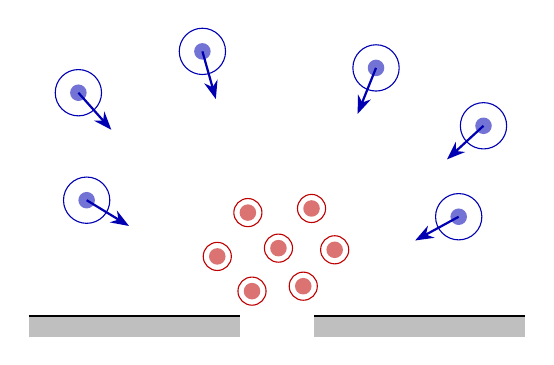
\begin{tikzpicture}[scale=1.05, >=Stealth]
        \fill[black!25] (-3,-0.25) rectangle (-0.45,0);
        \fill[black!25] (0.45,-0.25) rectangle (3,0);
        \draw[thick] (-3,0) -- (-0.45,0);
        \draw[thick] (0.45,0) -- (3,0);
        \foreach \x/\y in {-2.4/2.7, -0.9/3.2, 1.2/3.0, 2.5/2.3, -2.3/1.4, 2.2/1.2}
          {\agente{ev}{\x}{\y}{0.28}
           \draw[->,ev,thick] (\x,\y) -- ($(\x,\y)!0.6cm!(0,0)$);}
        \foreach \x/\y in {-0.3/0.3, 0.32/0.36, -0.72/0.72, 0.02/0.82, 0.7/0.8, -0.35/1.25, 0.42/1.3}
          {\agente{ts}{\x}{\y}{0.17}}
      \end{tikzpicture}
    \end{column}
  \end{columns}
\end{frame}

% CPM: reglas del modelo. El avance x(t + Δt) = x + v Δt y el orden del paso van en
% Implementación (devolución TP4, D6). Sin oraciones en las definiciones (devolución TP3, D4).
\begin{frame}{Modelo: radio y velocidad deseada}
  \begin{columns}[c]
    \begin{column}{0.60\textwidth}
      \setlength{\abovedisplayskip}{4pt}\setlength{\belowdisplayskip}{4pt}
      \textbf{Velocidad deseada}
      \[
        \vect{v}^{d}_i = v_d(r_i)\,\hat{\vect{e}}^{\,t}_i, \qquad
        \hat{\vect{e}}^{\,t}_i = \frac{\vect{x}^{t}_i - \vect{x}_i}{|\vect{x}^{t}_i - \vect{x}_i|}
      \]
      \[
        v_d(r_i) = \vdmax\left(\frac{r_i - \rmin}{\rmax - \rmin}\right)^{\beta}
      \]
      \vspace{0.6em}
      \textbf{Radio}
      \[
        r_i \leftarrow
        \begin{cases}
          \rmin & \text{con contacto}\\[0.2em]
          \min(r_i + \Delta r,\ \rmax) & \text{sin contacto}
        \end{cases}
      \]
      \[
        \Delta r = \frac{\rmax\,\Delta t}{\tau}, \qquad
        \Delta t = \frac{\rmin}{2\max(\vdmax, v_e)}
      \]
    \end{column}
    \begin{column}{0.38\textwidth}
      \centering
      % Cuerpo (r_min), espacio personal (r), target y dirección deseada.
      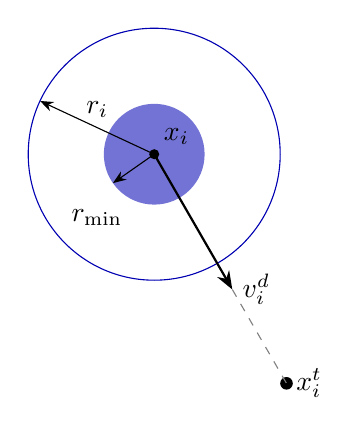
\begin{tikzpicture}[scale=3.2, >=Stealth]
        \draw[ev] (0,0) circle (0.5);
        \fill[ev!55] (0,0) circle (0.2);
        \draw[->] (0,0) -- (155:0.5) node[midway, above] {$r_i$};
        \draw[->] (0,0) -- (215:0.2);
        \node at (228:0.34) {$\rmin$};
        \draw[->, thick] (0,0) -- (-60:0.62) node[right] {$\vect{v}^{d}_i$};
        \fill (-60:1.05) circle (0.025) node[right] {$\vect{x}^{t}_i$};
        \draw[dashed, black!50] (-60:0.62) -- (-60:1.05);
        \fill (0,0) circle (0.02) node[above right] {$\vect{x}_i$};
      \end{tikzpicture}
    \end{column}
  \end{columns}
  \fuente{Baglietto y Parisi, Phys. Rev. E 83, 056117 (2011).}
\end{frame}

% Contacto con otro agente y con una pared (devolución TP4, D6: faltaban las ecuaciones de choque
% con paredes). x_j de una pared = punto más cercano p_i.
\begin{frame}{Modelo: contacto y escape}
  \begin{columns}[c]
    \begin{column}{0.58\textwidth}
      \setlength{\abovedisplayskip}{4pt}\setlength{\belowdisplayskip}{4pt}
      \textbf{Contacto con un agente y con una pared}
      \[
        |\vect{x}_i - \vect{x}_j| < r_i + r_j
      \]
      \[
        |\vect{x}_i - \vect{p}_i| < r_i, \qquad
        \vect{p}_i = \arg\min_{\vect{p}\,\in\,\text{pared}} |\vect{x}_i - \vect{p}|
      \]
      \vspace{0.3em}
      \textbf{Velocidad de escape}
      \[
        \vect{v}^{e}_i = v_e\,\frac{\sum_j \hat{\vect{e}}_{ij}}{\bigl|\sum_j \hat{\vect{e}}_{ij}\bigr|},
        \qquad
        \hat{\vect{e}}_{ij} = \frac{\vect{x}_i - \vect{x}_j}{|\vect{x}_i - \vect{x}_j|}
      \]
      \vspace{0.3em}
      \textbf{Velocidad}
      \[
        \vect{v}_i =
        \begin{cases}
          \vect{v}^{e}_i & \text{con contacto}\\[0.2em]
          \vect{v}^{d}_i & \text{sin contacto}
        \end{cases}
      \]
    \end{column}
    \begin{column}{0.36\textwidth}
      \centering
      % Dos agentes con los espacios personales superpuestos y una pared con su punto más cercano.
      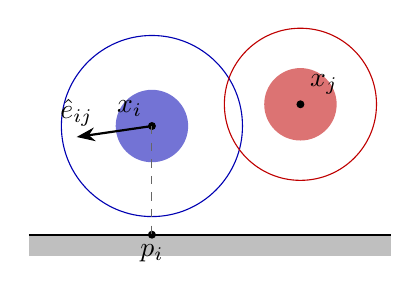
\begin{tikzpicture}[scale=2.3, >=Stealth]
        \fill[black!25] (-1.0,-0.72) rectangle (1.0,-0.6);
        \draw[thick] (-1.0,-0.6) -- (1.0,-0.6);
        \draw[ev] (-0.32,0) circle (0.5);
        \fill[ev!55] (-0.32,0) circle (0.2);
        \draw[ts] (0.5,0.12) circle (0.42);
        \fill[ts!55] (0.5,0.12) circle (0.2);
        \fill (-0.32,0) circle (0.022) node[above left] {$\vect{x}_i$};
        \fill (0.5,0.12) circle (0.022) node[above right] {$\vect{x}_j$};
        \draw[->, thick] (-0.32,0) -- ++(188.3:0.42) node[above] {$\hat{\vect{e}}_{ij}$};
        \fill (-0.32,-0.6) circle (0.022) node[below] {$\vect{p}_i$};
        \draw[dashed, black!60] (-0.32,0) -- (-0.32,-0.6);
      \end{tikzpicture}
    \end{column}
  \end{columns}
\end{frame}

% ==========================================================================
\section{Implementación}
% Solo el motor. Tres esquemas sobre las mismas reglas del CPM.
% ==========================================================================

% Paso temporal: las cuatro iteraciones del paper (sincrónicas) + cuerpo impenetrable + mover.
\begin{frame}{Paso temporal}
  \centering
  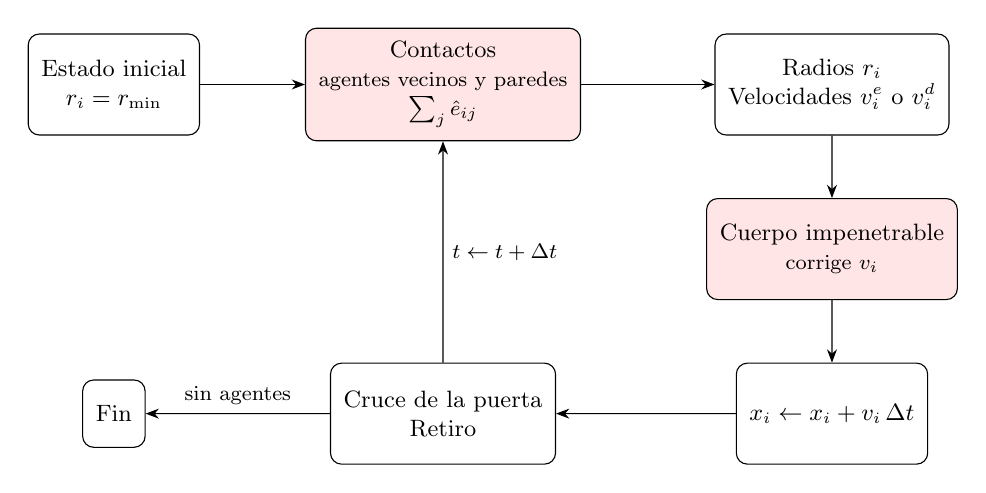
\begin{tikzpicture}[>=Stealth, font=\small, scale=0.95, every node/.append style={scale=0.95},
      caja/.style={draw, rounded corners, align=center, inner sep=5pt, minimum height=1.35cm},
      clave/.style={caja, fill=red!10}]
    \node[caja]  (ini)  at (0, 0)      {Estado inicial\\ $r_i = \rmin$};
    \node[clave] (con)  at (4.4, 0)    {Contactos\\ {\footnotesize agentes vecinos y paredes}\\
                                        {\footnotesize $\sum_j \hat{\vect{e}}_{ij}$}};
    \node[caja]  (rad)  at (9.6, 0)    {Radios $r_i$\\ Velocidades $\vect{v}^{e}_i$ o $\vect{v}^{d}_i$};
    \node[clave] (cue)  at (9.6, -2.2) {Cuerpo impenetrable\\ {\footnotesize corrige $\vect{v}_i$}};
    \node[caja]  (mov)  at (9.6, -4.4) {$\vect{x}_i \leftarrow \vect{x}_i + \vect{v}_i\,\Delta t$};
    \node[caja]  (fas)  at (4.4, -4.4) {Cruce de la puerta\\ Retiro};
    \node[caja, minimum height=0.9cm] (fin) at (0, -4.4) {Fin};
    \draw[->] (ini) -- (con);
    \draw[->] (con) -- (rad);
    \draw[->] (rad) -- (cue);
    \draw[->] (cue) -- (mov);
    \draw[->] (mov) -- (fas);
    \draw[->] (fas) -- node[right, font=\footnotesize] {$t \leftarrow t + \Delta t$} (con);
    \draw[->] (fas) -- node[above, font=\footnotesize] {sin agentes} (fin);
  \end{tikzpicture}
\end{frame}

% La diapositiva del cuerpo impenetrable (agregado propio: restricciones v_i·e_ij >= -(d_ij -
% 2 r_min)/(2 Δt) y v_i·e_ip >= -(d_ip - r_min)/Δt) se sacó (pedido 2026-11-10). Declararlo en
% vivo sobre el recuadro "Cuerpo impenetrable" del diagrama anterior: no es parte del CPM del paper.

% Eventos: entre eventos, MRU con radio constante. Estados de un agente; solo el diagrama (pedido
% 2026-11-10: sin la lista de eventos al costado).
% Dicho en vivo: los eventos son el contacto con un agente o una pared, el fin de escape, el fin de
% cada tramo de recuperación, el cambio de target y el retiro. Un contacto durante el escape o la
% recuperación reinicia el escape; cada escape dura Δt > 0, así que no hay cadenas en tiempo cero.
\begin{frame}{Eventos: estados de un agente}
  \centering
  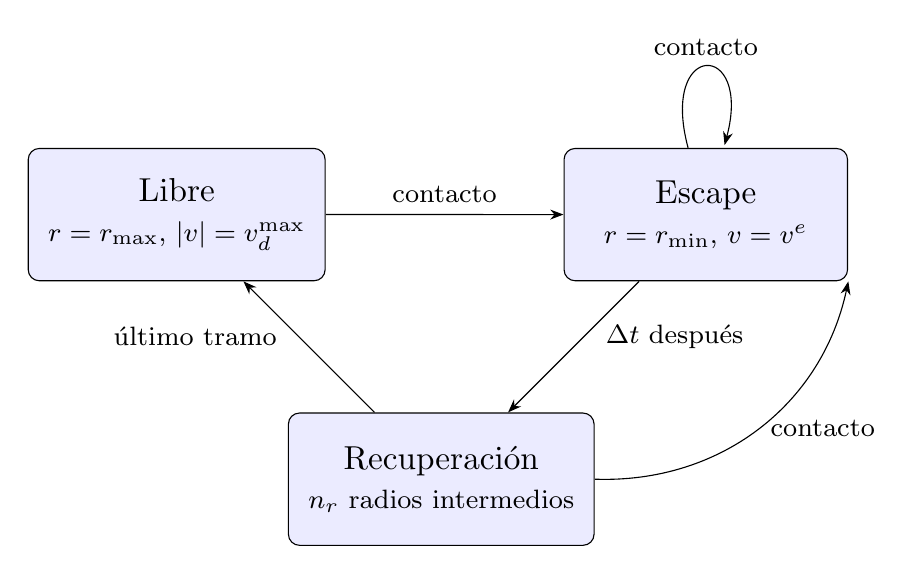
\begin{tikzpicture}[>=Stealth, scale=1.2, transform shape,
      est/.style={draw, rounded corners, align=center, inner sep=6pt, minimum height=1.4cm,
                  minimum width=3.0cm, fill=blue!8}]
    \node[est] (lib) at (0, 2.2)   {Libre\\ {\footnotesize $r = \rmax$, $|\vect{v}| = \vdmax$}};
    \node[est] (esc) at (5.6, 2.2) {Escape\\ {\footnotesize $r = \rmin$, $\vect{v} = \vect{v}^{e}$}};
    \node[est] (rec) at (2.8, -0.6) {Recuperación\\ {\footnotesize $n_r$ radios intermedios}};
    \draw[->] (lib) -- node[above, font=\footnotesize] {contacto} (esc);
    \draw[->] (esc) -- node[pos=0.42, right=3pt, font=\footnotesize] {$\Delta t$ después} (rec);
    \draw[->] (rec) -- node[pos=0.58, left=3pt, font=\footnotesize] {último tramo} (lib);
    \draw[->] (rec.east) to[bend right=40] node[right, font=\footnotesize] {contacto} (esc.south east);
    \path[->] (esc) edge[loop above] node[above, font=\footnotesize] {contacto} (esc);
  \end{tikzpicture}
\end{frame}

% La regla de contacto es la del CPM (siempre r_min y escape, como en paso temporal); lo propio de
% eventos es CUÁNDO se aplica: en el instante exacto t_c en que se tocan los espacios personales, y
% no al comienzo del paso siguiente. Dicho en vivo: se toma la menor raíz positiva; la regla se
% aplica a todos los agentes en contacto en ese instante; los cuerpos nunca se superponen porque
% el contacto salta cuando se tocan los espacios personales. (En el motor esto se llama "colapso".)
\begin{frame}{Eventos: instante del contacto}
  \begin{columns}[c]
    \begin{column}{0.58\textwidth}
      \setlength{\abovedisplayskip}{4pt}\setlength{\belowdisplayskip}{4pt}
      \textbf{Instante $t_c$ del contacto}
      \[
        \bigl|\Delta\vect{x}_{ij} + \Delta\vect{v}_{ij}\,t_c\bigr| = r_i + r_j
        \qquad\qquad
        \bigl|\vect{x}_i + \vect{v}_i\,t_c - \vect{p}_i\bigr| = r_i
      \]
      \vspace{0.6em}
      \textbf{En $t_c$: regla de contacto del modelo}
      \[
        r_i \leftarrow \rmin, \qquad
        \vect{v}_i \leftarrow \vect{v}^{e}_i
        \quad \text{durante } \Delta t
      \]
    \end{column}
    \begin{column}{0.40\textwidth}
      \centering
      % Arriba: justo antes de t_c, los espacios personales se tocan. Abajo: justo después, los
      % dos en r_min (solo el cuerpo) y escapando.
      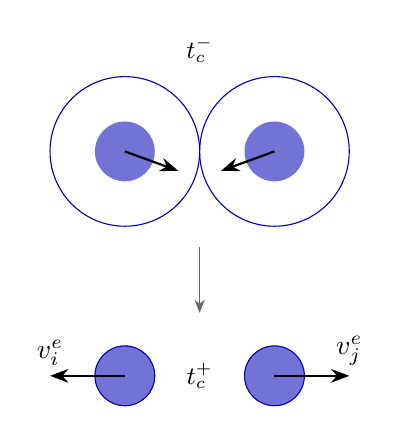
\begin{tikzpicture}[scale=1.9, >=Stealth]
        \foreach \x in {-0.5, 0.5}
          {\draw[ev] (\x,1.5) circle (0.5); \fill[ev!55] (\x,1.5) circle (0.2);}
        \draw[->, thick] (-0.5,1.5) -- ++(-20:0.38);
        \draw[->, thick] (0.5,1.5) -- ++(200:0.38);
        \node[font=\small] at (0,2.18) {$t_c^{-}$};
        \draw[->, black!60] (0,0.86) -- (0,0.42);
        \foreach \x in {-0.5, 0.5}
          {\fill[ev!55] (\x,0) circle (0.2); \draw[ev] (\x,0) circle (0.2);}
        \draw[->, thick] (-0.5,0) -- ++(180:0.5) node[above] {$\vect{v}^{e}_i$};
        \draw[->, thick] (0.5,0) -- ++(0:0.5) node[above] {$\vect{v}^{e}_j$};
        \node[font=\small] at (0,0) {$t_c^{+}$};
      \end{tikzpicture}
    \end{column}
  \end{columns}
\end{frame}

% Parámetro propio con nombre y ejemplos dibujados (como D11-D13 del TP3; pedido 2026-11-10: con
% dibujos y no con un gráfico). A escala: 1 cm = 0.29 m (r_min 0.34 cm, r_1 0.40 cm, r_2 0.45 cm,
% r_max 0.85 cm); flechas de velocidad 0.7 cm por m/s (v_e = v_dmax = 1.5; v_d(r_1) = 0.21;
% v_d(r_2) = 0.39 m/s). Debajo de cada estado: radio y cuánto dura.
% Dicho en vivo: con n_r = 0 el agente queda quieto en r_min hasta 9 Δt después del contacto y
% vuelve de golpe a r_max; con n_r = 2 recorre los dos primeros radios de paso temporal y sostiene
% el segundo; con n_r = 8 recorre los mismos radios que paso temporal. Al empezar un tramo el radio
% salta: si pisa a un vecino, hay contacto en ese instante.
\begin{frame}{Eventos: recuperación con $n_r$ radios intermedios}
  \centering
  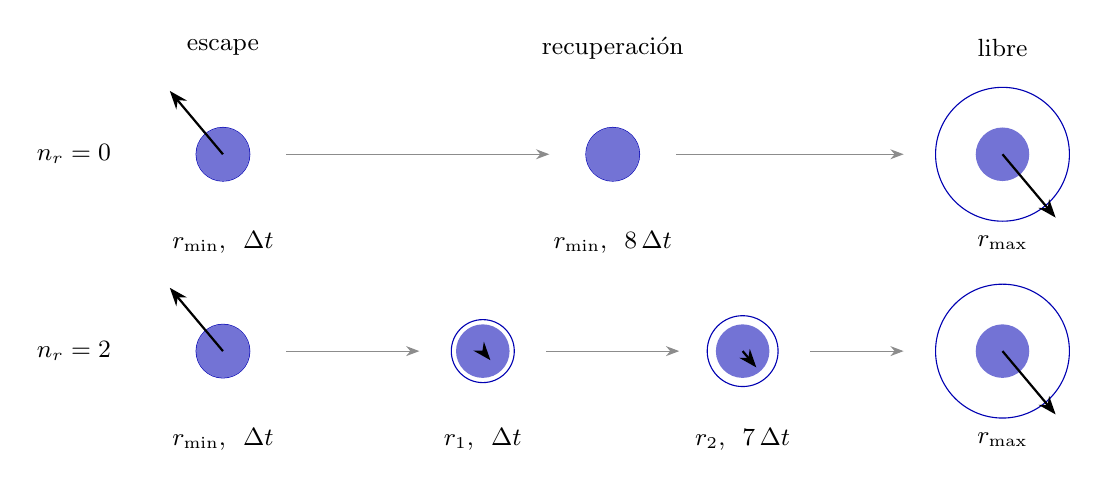
\begin{tikzpicture}[>=Stealth, font=\small,
      paso/.style={->, black!45, shorten >=3pt, shorten <=3pt}]
    \node at (0,1.35) {escape};
    \node at (4.95,1.35) {recuperación};
    \node at (9.9,1.35) {libre};
    % n_r = 0
    \node[left] at (-1.3,0) {$n_r = 0$};
    \estado{0}{0}{0.34}{130}{1.05}{$\rmin$, \ $\Delta t$}
    \estado{4.95}{0}{0.34}{0}{0}{$\rmin$, \ $8\,\Delta t$}
    \estado{9.9}{0}{0.85}{-50}{1.05}{$\rmax$}
    \draw[paso] (0.7,0) -- (4.25,0);
    \draw[paso] (5.65,0) -- (8.75,0);
    % n_r = 2
    \begin{scope}[yshift=-2.5cm]
      \node[left] at (-1.3,0) {$n_r = 2$};
      \estado{0}{0}{0.34}{130}{1.05}{$\rmin$, \ $\Delta t$}
      \estado{3.3}{0}{0.40}{-50}{0.15}{$r_1$, \ $\Delta t$}
      \estado{6.6}{0}{0.45}{-50}{0.27}{$r_2$, \ $7\,\Delta t$}
      \estado{9.9}{0}{0.85}{-50}{1.05}{$\rmax$}
      \draw[paso] (0.7,0) -- (2.6,0);
      \draw[paso] (4.0,0) -- (5.9,0);
      \draw[paso] (7.35,0) -- (8.75,0);
    \end{scope}
  \end{tikzpicture}
  \vspace{0.2em}
  \[
    r_k = \rmin + k\,\Delta r, \qquad |\vect{v}| = v_d(r_k), \qquad k = 1, \dots, n_r
  \]
\end{frame}

% Híbrido: criterio de pasaje. D = max(R_h, 2 r_max): un agente en eventos pasa antes de tocar a
% uno en paso temporal. Dicho en vivo: el pasaje se hace en el próximo paso de la grilla, con el
% radio que tenga el agente, y arrastra a los agentes en eventos que queden a menos de D.
\begin{frame}{Híbrido: criterio de pasaje con el área $R_h$}
  \begin{columns}[c]
    \begin{column}{0.44\textwidth}
      \centering
      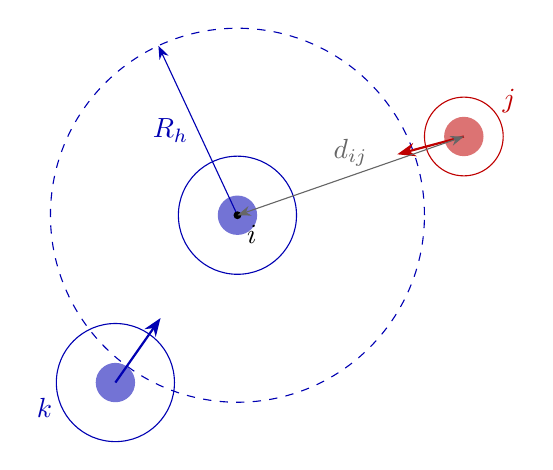
\begin{tikzpicture}[scale=2.5, >=Stealth]
        \draw[ev, dashed] (0,0) circle (0.95);
        \agente{ev}{0}{0}{0.3}
        \draw[->, ev] (0,0) -- (115:0.95) node[midway, left] {$R_h$};
        \fill (0,0) circle (0.02) node[below right] {$i$};
        \agente{ev}{-0.62}{-0.85}{0.3}
        \draw[->, ev, thick] (-0.62,-0.85) -- ++(55:0.4);
        \node[ev] at (-0.98,-0.98) {$k$};
        \agente{ts}{1.15}{0.4}{0.2}
        \draw[->, ts, thick] (1.15,0.4) -- ++(195:0.35);
        \node[ts] at (1.38,0.58) {$j$};
        \draw[<->, black!60] (0,0) -- (1.15,0.4) node[midway, above] {$d_{ij}$};
      \end{tikzpicture}
    \end{column}
    \begin{column}{0.54\textwidth}
      \setlength{\abovedisplayskip}{4pt}\setlength{\belowdisplayskip}{4pt}
      \textbf{Eventos $\to$ paso temporal:} alguna
      \begin{align*}
        d_{ik} &\le R_h && (k \text{ en eventos})\\
        d_{ij} &\le D = \max(R_h,\ 2\,\rmax) && (j \text{ en paso temporal})\\
        d_{ip} &\le \tfrac{1}{2} R_h && (\text{pared})
      \end{align*}
      \vspace{0.3em}
      \textbf{Paso temporal $\to$ eventos:} todas
      \begin{align*}
        r_i &= \rmax, \ \text{sin contacto}\\
        d_{ij} &> D \quad \forall j\\
        d_{ip} &> \tfrac{1}{2} D
      \end{align*}
    \end{column}
  \end{columns}
\end{frame}

% Convivencia: grilla global t_n = n Δt. Dicho en vivo: dentro de un paso el agente en paso
% temporal tiene velocidad constante, así que su llegada a distancia D de un agente en eventos se
% predice con la misma cuadrática; esa predicción vale hasta t_{n+1}.
\begin{frame}{Híbrido: sincronización entre eventos y pasos}
  \centering
  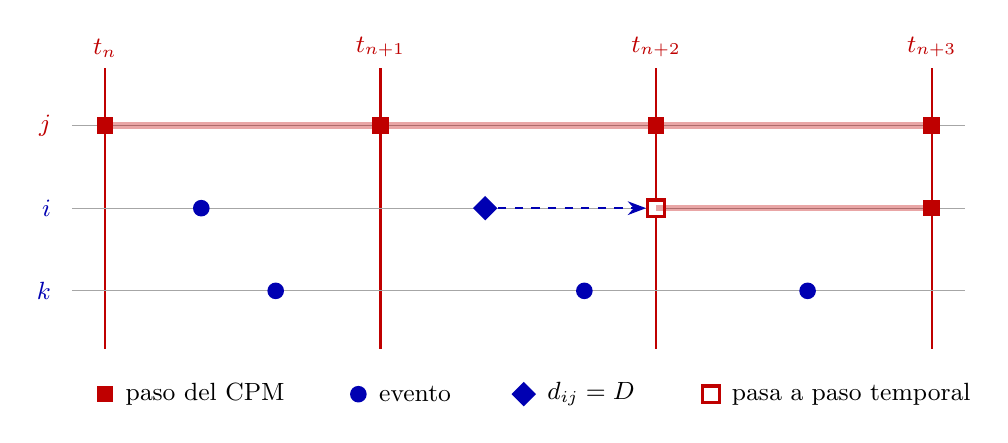
\begin{tikzpicture}[>=Stealth, font=\small, x=3.5cm, y=1.05cm]
    \foreach \k/\lab in {0/t_n, 1/t_{n+1}, 2/t_{n+2}, 3/t_{n+3}}
      {\draw[ts, thick] (\k,0.3) -- (\k,3.7) node[above] {$\lab$};}
    \foreach \y/\lab/\c in {3/j/ts, 2/i/ev, 1/k/ev}
      {\draw[black!35] (-0.12,\y) -- (3.12,\y); \node[left, \c] at (-0.16,\y) {$\lab$};}
    % j: paso temporal en todos los pasos
    \draw[ts, line width=2.4pt, opacity=0.35] (0,3) -- (3,3);
    \foreach \k in {0,1,2,3} {\node[fill=ts, minimum size=6pt, inner sep=0pt] at (\k,3) {};}
    % i: eventos; llega a distancia D de j y pasa en el paso siguiente
    \fill[ev] (0.35,2) circle (3pt);
    \node[diamond, fill=ev, minimum size=9pt, inner sep=0pt] (near) at (1.38,2) {};
    \node[draw=ts, very thick, fill=white, minimum size=6pt, inner sep=0pt] (pass) at (2,2) {};
    \draw[->, ev, dashed, thick] (near) -- (pass);
    \draw[ts, line width=2.4pt, opacity=0.35] (2,2) -- (3,2);
    \node[fill=ts, minimum size=6pt, inner sep=0pt] at (3,2) {};
    % k: solo eventos
    \foreach \x in {0.62, 1.74, 2.55} {\fill[ev] (\x,1) circle (3pt);}
    % referencias
    \begin{scope}[shift={(0,-0.25)}]
      \node[fill=ts, minimum size=6pt, inner sep=0pt] at (0.0,0) {};
      \node[right] at (0.04,0) {paso del CPM};
      \fill[ev] (0.92,0) circle (3pt);
      \node[right] at (0.96,0) {evento};
      \node[diamond, fill=ev, minimum size=9pt, inner sep=0pt] at (1.52,0) {};
      \node[right] at (1.57,0) {$d_{ij} = D$};
      \node[draw=ts, very thick, fill=white, minimum size=6pt, inner sep=0pt] at (2.2,0) {};
      \node[right] at (2.24,0) {pasa a paso temporal};
    \end{scope}
  \end{tikzpicture}
\end{frame}

% Lazo del híbrido. En azul lo que es por eventos, en rojo lo que es por paso temporal.
\begin{frame}{Híbrido: motor}
  \centering
  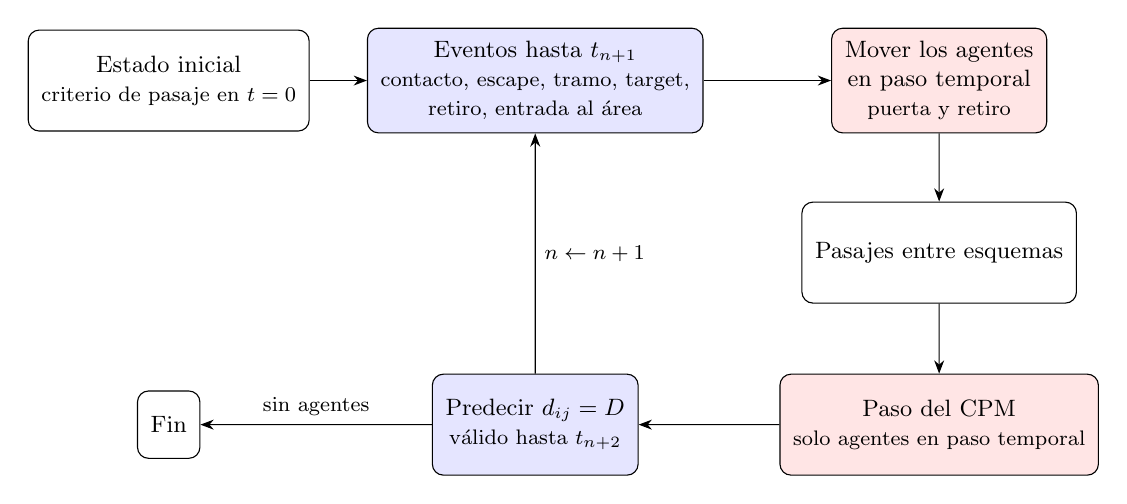
\begin{tikzpicture}[>=Stealth, font=\small, scale=0.95, every node/.append style={scale=0.95},
      caja/.style={draw, rounded corners, align=center, inner sep=5pt, minimum height=1.35cm},
      cev/.style={caja, fill=blue!10}, cts/.style={caja, fill=red!10}]
    \node[caja] (ini)  at (0, 0)      {Estado inicial\\ {\footnotesize criterio de pasaje en $t = 0$}};
    \node[cev]  (eve)  at (4.9, 0)    {Eventos hasta $t_{n+1}$\\
                                       {\footnotesize contacto, escape, tramo, target,}\\
                                       {\footnotesize retiro, entrada al área}};
    \node[cts]  (mov)  at (10.3, 0)   {Mover los agentes\\ en paso temporal\\
                                       {\footnotesize puerta y retiro}};
    \node[caja] (pas)  at (10.3, -2.3) {Pasajes entre esquemas};
    \node[cts]  (cpm)  at (10.3, -4.6) {Paso del CPM\\ {\footnotesize solo agentes en paso temporal}};
    \node[cev]  (pre)  at (4.9, -4.6)  {Predecir $d_{ij} = D$\\ {\footnotesize válido hasta $t_{n+2}$}};
    \node[caja, minimum height=0.9cm] (fin) at (0, -4.6) {Fin};
    \draw[->] (ini) -- (eve);
    \draw[->] (eve) -- (mov);
    \draw[->] (mov) -- (pas);
    \draw[->] (pas) -- (cpm);
    \draw[->] (cpm) -- (pre);
    \draw[->] (pre) -- node[right, font=\footnotesize] {$n \leftarrow n + 1$} (eve);
    \draw[->] (pre) -- node[above, font=\footnotesize] {sin agentes} (fin);
  \end{tikzpicture}
\end{frame}

% Valores característicos de R_h (el parámetro principal del criterio, punto c) y garantía de que
% no se pierden contactos. Dicho en vivo: por debajo de 2 r_min nadie puede entrar al área de otro
% (los cuerpos lo impiden) y la corrida es idéntica a eventos puro; desde 2 r_max + 2 v Δt el
% pasaje llega siempre antes que el contacto.
\begin{frame}{Híbrido: valores de $R_h$ y contactos}
  \centering
  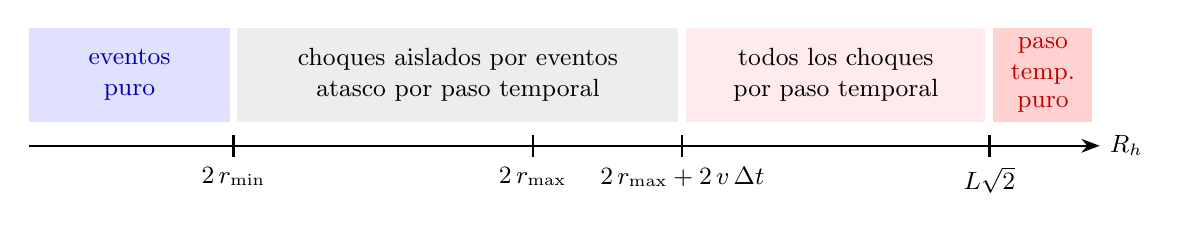
\begin{tikzpicture}[>=Stealth, font=\small, x=1.0cm, y=1.0cm]
    \draw[->, thick] (0,0) -- (13.6,0) node[right] {$R_h$};
    \foreach \x/\lab in {2.6/{2\,\rmin}, 6.4/{2\,\rmax}, 8.3/{2\,\rmax + 2\,v\,\Delta t}, 12.2/{L\sqrt{2}}}
      {\draw[thick] (\x,0.14) -- (\x,-0.14) node[below] {$\lab$};}
    \fill[blue!12] (0,0.3) rectangle (2.55,1.5);
    \node[align=center, ev] at (1.28,0.9) {eventos\\ puro};
    \fill[black!7] (2.65,0.3) rectangle (8.25,1.5);
    \node[align=center] at (5.45,0.9) {choques aislados por eventos\\ atasco por paso temporal};
    \fill[red!8] (8.35,0.3) rectangle (12.15,1.5);
    \node[align=center] at (10.25,0.9) {todos los choques\\ por paso temporal};
    \fill[red!18] (12.25,0.3) rectangle (13.5,1.5);
    \node[align=center, ts] at (12.88,0.9) {paso\\ temp.\\[-0.1em] puro};
  \end{tikzpicture}
  \vspace{1.2em}

  \setlength{\abovedisplayskip}{4pt}\setlength{\belowdisplayskip}{4pt}
  \textbf{Sin contactos perdidos ni cuerpos superpuestos}
  \begin{columns}[T]
    \begin{column}{0.36\textwidth}
      \centering
      Dos agentes en eventos\\[0.4em]
      el contacto es un evento
    \end{column}
    \begin{column}{0.60\textwidth}
      \centering
      Uno en eventos y uno en paso temporal
      \[
        d_{ij} \ \ge\ D - 2\,v\,\Delta t \ \ge\ 2\,\rmax - \rmin \ >\ 2\,\rmin
      \]
    \end{column}
  \end{columns}
\end{frame}

% ==========================================================================
\section{Simulaciones}
% Sistema particular, parámetros, observables. Sin resultados.
% ==========================================================================

% Puerta y distancia de retiro exageradas para que se vean. La condición inicial va aparte de los
% parámetros (devolución TP3, D8). Valores de cada barrido: se ven en cada figura.
\begin{frame}{Sistema}
  \begin{columns}[c]
    \begin{column}{0.46\textwidth}
      \centering
      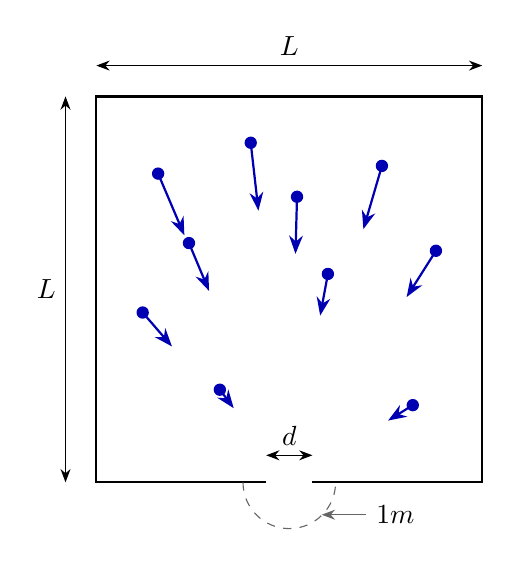
\begin{tikzpicture}[scale=0.098, >=Stealth]
        \draw[thick] (22,0) -- (0,0) -- (0,50) -- (50,50) -- (50,0) -- (28,0);
        \draw[<->] (-4,0) -- (-4,50) node[midway, left] {$L$};
        \draw[<->] (0,54) -- (50,54) node[midway, above] {$L$};
        \draw[<->] (22,3.5) -- (28,3.5) node[midway, above] {$d$};
        \draw[dashed, black!60] (19,0) arc[start angle=180, end angle=360, radius=6];
        \draw[<-, black!60] (29.2,-4.2) -- (35,-4.2) node[right, black] {$1\uni{m}$};
        \foreach \x/\y in {8/40, 20/44, 37/41, 44/30, 6/22, 30/27, 16/12, 41/10, 26/37, 12/31}
          {\fill[ev] (\x,\y) circle (0.8);
           \draw[->, ev, thick] (\x,\y) -- ($(\x,\y)!0.2!(25,0)$);}
      \end{tikzpicture}
    \end{column}
    \begin{column}{0.52\textwidth}
      \textbf{Parámetros fijos}\par
      \begin{minipage}[t]{0.47\linewidth}
        \begin{itemize}\setlength{\itemsep}{1pt}
          \item $d = 0.8\uni{m}$
          \item $\rmin = 0.10\uni{m}$
          \item $\rmax = 0.25\uni{m}$
          \item $\vdmax = 1.5\uni{m/s}$
        \end{itemize}
      \end{minipage}\hfill
      \begin{minipage}[t]{0.51\linewidth}
        \begin{itemize}\setlength{\itemsep}{1pt}
          \item $v_e = 1.5\uni{m/s}$
          \item $\beta = 0.9$
          \item $\tau = 0.5\uni{s}$
          \item $\Delta t = 1/30\uni{s}$
        \end{itemize}
      \end{minipage}\par
      \vspace{0.4em}
      \textbf{Parámetros variables}
      \begin{itemize}\setlength{\itemsep}{1pt}
        \item $R_h$ entre $0.1$ y $10\uni{m}$; \ $n_r$ entre 0 y 8
        \item $N$ entre 100 y 1000 (base: 500)
        \item $L$ entre 22 y $300\uni{m}$ (base: 50)
      \end{itemize}
      \vspace{0.2em}
      \textbf{Condición inicial}
      \begin{itemize}\setlength{\itemsep}{1pt}
        \item Posiciones al azar sin superposición; $r_i = \rmin$
      \end{itemize}
    \end{column}
  \end{columns}
\end{frame}

% Observables. La curva de población cuenta cruces de la puerta ("dentro de la habitación"); el
% tiempo de evacuación es el último retiro (decisión del grupo, 2026-11-10): la curva llega a 0
% unos 0.9 s antes. Caudal: ventana provisoria entre el 20 % y el 80 % de los cruces.
% TODO: justificar la ventana del caudal sobre la curva de población (o sacar el caudal).
\begin{frame}{Observables}
  \begin{columns}[c]
    \begin{column}{0.58\textwidth}
      \begin{itemize}\setlength{\itemsep}{0.6em}
        \item $N_{in}(t)$: agentes que todavía no cruzaron la puerta.
        \item $t_{ev}$: instante en que se retira el último agente.\\[0.2em]
          $t_{90}$: instante en que se retiró el 90\,\%.
        \item Caudal: $Q = \dfrac{0.6\,N}{t_{80} - t_{20}}$
        \item Tiempo de ejecución del lazo de simulación.
        \item Promedio y desvío estándar sobre 10 realizaciones.
      \end{itemize}
    \end{column}
    \begin{column}{0.40\textwidth}
      \centering
      % Curva de población esquemática: cruces 20 % y 80 % para el caudal, y t_ev.
      \begin{tikzpicture}[x=0.040cm, y=0.040cm, >=Stealth, font=\small]
        \draw[->] (0,0) -- (106,0) node[below] {$t$};
        \draw[->] (0,0) -- (0,114) node[above] {$N_{in}$};
        \draw[thick] (0,100) -- (6,100) -- (88,0);
        \draw[dashed, black!55] (0,80) -- (22.4,80) -- (22.4,0) node[below, black] {$t_{20}$};
        \draw[dashed, black!55] (0,20) -- (71.6,20) -- (71.6,0) node[below, black] {$t_{80}$};
        \node[left] at (0,100) {$N$};
        \node[left] at (0,80) {$0.8\,N$};
        \node[left] at (0,20) {$0.2\,N$};
        \draw[ts, thick] (93,-3) -- (93,3) node[above] {$t_{ev}$};
      \end{tikzpicture}
    \end{column}
  \end{columns}
\end{frame}

% ==========================================================================
\section{Resultados}
% Por estudio: animación -> evolución temporal -> input vs observable.
% ==========================================================================

% --- Los tres esquemas (puntos a y b) --------------------------------------

% TODO: generar y subir. Propuesta del grupo: eventos con n_r = 0 y paso temporal; misma tasa de
%   cuadros por segundo simulado en las dos (devolución TP4, D19). Eventos: un cuadro cada k
%   eventos (sin interpolar, devolución TP3).
\begin{frame}{Esquemas: animaciones de eventos y de paso temporal}
  \animdos{anim_eventos_nr0.png}{Eventos, $n_r = 0$}{enlace pendiente}
          {anim_paso_temporal.png}{Paso temporal}{enlace pendiente}
\end{frame}

% Pedido 2026-11-10: después de las animaciones de eventos, el tiempo de ejecución según n_r; sin
% texto al costado (la leyenda de la figura ya nombra la recta de trazos; lo demás se dice en vivo).
% Dicho en vivo (N = 500): 9.5-9.7 s con n_r de 1 a 8, o sea que no depende de n_r; con n_r = 0,
% 6.8 ± 0.2 s, pero solo evacuaron 7 de las 10 realizaciones (las otras 3 se cortaron con 2 agentes
% trabados y no entran en el promedio). Paso temporal: 0.88 ± 0.03 s.
% Las otras dos diapositivas de n_r (t_90 y caudal) siguen más abajo, después de la comparación de
% esquemas: decidir si se traen acá para que el estudio de n_r quede junto.
\begin{frame}{Radios intermedios: tiempo de ejecución vs $n_r$}
  \figura{campaign/eventos_ejecucion_vs_niveles.png}
\end{frame}

% TODO: decidir los dos R_h (propuesta: 0.5 m con L = 50 m, y uno con L = 300 m, donde el híbrido
%   gana). Agentes coloreados por esquema: azul eventos, rojo paso temporal.
\begin{frame}{Esquemas: animaciones del híbrido}
  \animdos{anim_hibrido_1.png}{Híbrido, $R_h$ a definir}{enlace pendiente}
          {anim_hibrido_2.png}{Híbrido, $R_h$ a definir}{enlace pendiente}
\end{frame}

% Punto a: fracción de los N agentes en cada esquema vs t. Una corrida (seed 1), N = 500, L = 50 m.
% Dicho en vivo: en t = 0 los 500 arrancan en eventos (nadie tiene a otro dentro del área); paso
% temporal supera a eventos desde t = 17.1 s y llega a 419 agentes en t = 31.1 s; 80 % de los
% pasos-agente son de paso temporal. Las dos curvas suman la fracción que todavía no se retiró.
\begin{frame}{Híbrido: agentes en cada esquema con $R_h = 0.5\uni{m}$}
  \figura{campaign/hibrido_agentes_por_esquema_N500_L50_rh0.5.png}
\end{frame}

% Punto b: evolución temporal del observable. Una sola corrida por esquema (seed 1; pedido
% 2026-11-10), para ver el comportamiento; los promedios van en las diapositivas siguientes.
% Híbrido con R_h = 0.5 m (cae sobre paso temporal). N = 500. Dicho en vivo, tiempo de evacuación de
% esa seed: 165.2 s (paso temporal), 253.3 s (eventos), 164.9 s (híbrido).
\begin{frame}{Esquemas: agentes en la habitación vs tiempo}
  \figura{campaign/poblacion_N500.png}
\end{frame}

% Dicho en vivo (N = 500): paso temporal 166.1 ± 1.4 s, eventos (n_r = 8) 255.9 ± 1.8 s, híbrido
% (R_h = 0.5 m) 165.2 ± 1.0 s.
\begin{frame}{Esquemas: tiempo de evacuación}
  \figura{campaign/evacuacion_esquemas.png}
\end{frame}

% Punto c (primera parte). Dicho en vivo (N = 500): 0.88 ± 0.03 s, 9.7 ± 0.2 s y 0.95 ± 0.03 s.
\begin{frame}{Esquemas: tiempo de ejecución}
  \figura{campaign/ejecucion_esquemas.png}
\end{frame}

% --- Radios intermedios de eventos (estudio propio) -------------------------

% t_90 y no t_ev: con n_r = 0 no evacuaron 3 de las 10 realizaciones (quedan 2 agentes trabados
% frente a la puerta: resultado válido según la cátedra).
% Dicho en vivo (N = 500): 1510 ± 50 s con n_r = 0, 280 ± 3 s con 1, 227-229 s de 4 a 8, contra
% 146.0 ± 1.4 s de paso temporal.
\begin{frame}{Radios intermedios: tiempo de salida del 90\,\% vs $n_r$}
  \figura{campaign/eventos_t90_vs_niveles.png}
\end{frame}

% Dicho en vivo (N = 500): 0.30, 1.64, 1.89, 1.98 y 2.00-2.02 1/s, contra 3.29 de paso temporal.
\begin{frame}{Radios intermedios: caudal vs $n_r$}
  \figura{campaign/eventos_caudal_vs_niveles.png}
\end{frame}

% --- Radio del área del híbrido (punto c) -----------------------------------

% Dicho en vivo (N = 500): con R_h = 0.1 m, 255.9 ± 1.8 s (las mismas corridas que eventos puro);
% desde 0.2 m, 165.0-166.2 s. La transición es brusca: el primer par que pasa a paso temporal
% arrastra a todo el atasco.
\begin{frame}{Radio del área: tiempo de evacuación vs $R_h$}
  \figuranota{campaign/hibrido_evacuacion_vs_rh_N500.png}{%
    Punteado: $2\,\rmin$ y $2\,\rmax$.}
\end{frame}

% Dicho en vivo (N = 500, L = 50 m): 9.72 ± 0.20 s con R_h = 0.1 m (eventos: 9.7 ± 0.2 s);
% 0.95-1.03 s desde 0.2 m, contra 0.88 ± 0.03 s de paso temporal.
\begin{frame}{Radio del área: tiempo de ejecución vs $R_h$}
  \figuranota{campaign/hibrido_ejecucion_vs_rh_N500.png}{%
    Punteado: $2\,\rmin$ y $2\,\rmax$.}
\end{frame}

% Estudio propio: N = 500 en habitaciones más grandes. Dicho en vivo: con L = 300 m el híbrido
% tarda 0.45 ± 0.03 s contra 0.69 ± 0.02 s de paso temporal y le gana hasta R_h ≈ 4 m; con
% L = 150 m, 0.71 contra 0.76 s y le gana hasta ≈ 1 m. Con R_h = 0.1 m (eventos puro): 9.7, 6.7 y
% 3.0 s, porque con L grande los agentes llegan más espaciados y el atasco es más chico.
\begin{frame}{Radio del área: tiempo de ejecución vs $R_h$ según $L$}
  \figura{campaign/hibrido_ejecucion_vs_rh_por_L_N500.png}
\end{frame}

% --- Número de agentes (punto d) ---------------------------------------------

% Dicho en vivo: exponente local (t ∝ N^α entre N consecutivos): eventos 2.2-2.6; paso temporal de
% 1.3 a 2.2; híbrido de 1.3 a 2.3. N = 1000: 3.80 ± 0.07 s, 51.5 ± 0.4 s y 4.0 ± 0.6 s.
% TODO: avisar los atascos de N = 1000 (paso temporal, seed 5, no evacuó; híbrido, seeds 5 y 6,
%   403 y 518 s contra ~312 s).
\begin{frame}{Número de agentes: tiempo de ejecución con $L = 50\uni{m}$}
  \figura{campaign/ejecucion_vs_N_L50.png}
\end{frame}

% Densidad inicial 0.2 agentes/m² (la del sistema base): L = 22.4 a 70.7 m.
\begin{frame}{Número de agentes: tiempo de ejecución a densidad constante}
  \figura{campaign/ejecucion_vs_N_densidad_constante.png}
\end{frame}

% ==========================================================================
\section{Conclusiones}
% Solo lo que está en las figuras de Resultados. Cuantificar.
% ==========================================================================

% Boceto: redactar con el grupo. Respaldo: tp5-pedestrian-dynamics/AGENTS.md §6.5 y §6.6.
\begin{frame}{Conclusiones}
  \begin{itemize}\setlength{\itemsep}{0.8em}
    \item Con $N = 500$, eventos evacúa en $256 \pm 2\uni{s}$ contra $166.1 \pm 1.4\uni{s}$ de
      paso temporal, y tarda 11 veces más en ejecutarse.
    \item En eventos, pasar de $n_r = 0$ a $1$ baja $\langle t_{90}\rangle$ de $1510$ a
      $280\uni{s}$; desde $n_r = 4$ no cambia, y no alcanza a paso temporal.
    \item El híbrido reproduce a eventos con $R_h < 2\,\rmin$ y a paso temporal desde
      $R_h = 2\,\rmin$: la transición es brusca.
    \item Con $L = 50\uni{m}$ el híbrido tarda 8\,\% más que paso temporal; con $L = 300\uni{m}$,
      35\,\% menos.
    \item El tiempo de ejecución crece como $N^{2.4}$ en eventos y como $N^{2}$ en paso temporal
      y en el híbrido para $N \ge 500$.
  \end{itemize}
\end{frame}

\begin{frame}[plain]
  \centering
  \vfill
  {\Huge Muchas gracias}
  \vfill
\end{frame}

\end{document}
